\section{Race and the Myth of the Origins of Rome I}

\begin{quotationx}
This essay by \textbf{Julius Evola} was originally published in the journal \emph{La Difesa della Razza}.

In the context of the recent series of posts, this can be understood as the ``Noble Lie" about the birth of Rome. From the point of view of profane history, these myths are simply superstitions. Evola, on the other hand, drawing on Vico, Bachofen, Guenon, \emph{inter alios}, views such symbols, myths, and legends as witnesses to the inner spirit of a people, which cannot be grasped simply in the accumulation of historical facts. Logically, this technique leads him to move beyond the merely physical and zoological understanding of race to the notion of the races of the soul and of the spirit. (This is a reformulation of the Rosicrucian notions of the folk soul and folk spirit.)

In this first part, Evola brings to light two aspects of the myth. First is the idea that the founder was born from the union of a god with a mortal woman. The god confers spiritual qualities on the founder. In this case, Mars, as the god-father of Romulus and Remus, is the spirit of warrior virility, not just on the twins, but on the entire city.

The second aspect is being saved from the Tiber as infants. For Evola, this represents the hero, the seer, etc., men above the flow of time.

The defect in Evola's methodology is that he is left in the same position as the profane historian: the third person perspective. Although he sees more deeply, he is still an outsider and does not participate in the myth. So, yes, for him, too, it is a Noble Lie. For the Romans, Mars was a living being, not some abstract force, and the story of their miraculous rescue from the Tiber was considered history, not legend.

Although we can get some idea of the spirituality and mentality of the Romans from Evola's analysis, a scholarly discussion cannot lead us to that same state. For that, the method of Hermetic meditation described by \textbf{Valentin Tomberg} is much more helpful\footnote{\url{https://www.gornahoor.net/?p=898}}. This is a lesson for those hoping to establish a new regime somewhere, sometime: they must create a noble lie that is also a spiritual truth. 

\end{quotationx}
In his \emph{Life of Romulus} (I,8), \textbf{Plutarch} writes:

\begin{quotex}
Rome would not have risen to such power had it not had, in any way, a divine origin, such as to offer to the eyes of men something great and inexplicable. 

\end{quotex}
\textbf{Cicero} repeats the same thing (Nat. Deor. II,3,8) and considered (Har. Resp., IX, 19) the Roman civilization as that which through sacred knowledge ``surpassed every other people and nation": \emph{omnes gentes nationesque superavivums}. Sallust called the ancient Romans \emph{religiosissimi mortales} [the most religious mortals].

On the other hand, in our day all of that is fantasy or superstition for many ``serious" persons and many ``critical" minds. The ``facts" are the only things that count for them. The mythical traditions of the ancients have no value, or they have it only insofar as it is supposed that, here and there, they are confused reflections of real events, that is to say, tangibly historical. There is, in that, a fundamental misunderstanding that was already denounced, to a certain degree by our \textbf{Giambattista Vico}, then by Schelling, still more recently by Bachofen and, finally, by the most recent school of the metaphysical interpretation of myth, and by those little known today (Guenon, W. R. Otto, Altheim, Kerenyi, etc.). According to all these writers, the mystical traditions are neither arbitrary creations more or less on the poetic and fantastic plane, nor deformations and transpositions of historical elements. Especially in regard to origins, it was correctly pointed out that symbols and legends,

\begin{quotex}
if only in a dramatized form, represent actually and truly the history of the beginnings of a nation, but not the history of events occurring materially on earth, but rather of spiritual processes that have given birth to a new people alongside other people although different in culture and civilization: history, so to say, of its prenatal period.

Legend and history are tightly connected; the former proceeds through interiorization and is dispersed through images, while the latter proceeds through exteriorization as facts and events. These images are the result of formative living forces, facts are organized by the human thought. In legends one is transported by formative forces; in the other, there is premeditated organization of facts. But the legend is the invisible part and root of history; it is not poetry, rather it is a reality much vaster than history itself. The threads of the destiny of a people that unravel visibly in the most various ways in their historical development, go back to the impulses, to the creative spheres, to which the heroes of its legends are connected. 

\end{quotex}
In a particular way, \textbf{Bachofen} revealed that even at the point in which evidence, by being recognized as a myth, came to be rejected by profane history, even when it is a positive witness to the spirit of a people.

In that way, a study of mythical traditions, using new criteria, can lead us to interesting conclusions from the point of view of a theory of race that is not defined by the material aspects of the issues, but also addresses the inner reality of race.

On the occasion of the current anniversary of the Birth of Rome, we want to illustrate this interpretative method, applying it precisely to the exegesis of the myth of our origins. The legends related to the birth of Rome concentrate such a quantity of sensitive elements based on general meanings of civilizations and mythologies of Aryan peoples, that a special work would be necessary to analyze them and clarify them adequately. Therefore, we will point out here only the most notable themes, among which are: the miraculous birth, the theme of being ``saved by the waters", the ``wolf", the ``tree", the rival pair of twins.

The myth of the union of a god with a mortal woman, in the present case, of Mars with Rhea Silvia, from which union Romulus and Remus were born, recurs in almost all traditions in regard to the birth of ``divine heroes". Zeus and Leto gave birth to Apollo, Zeus and Alcmene to Hercules, Heracles being the symbolic hero of the Doric-Achaean Aryan peoples, and Apollo having a connection with the land of the Hyperboreans and with the primordial Nordic-Aryan races. An analogous origin, in properly Germanic traditions, is attributed to the heroic peoples of the Volsungs, to which Siegfried belongs.

In the ancient royal Egyptian tradition — whose remote origin can with good reason also be considered to be Aryan, Atlantic-Occidental — every sovereign is thought to have been begotten by a god uniting with the queen: this tradition in which the hidden meaning of the myth comes to the fore, inasmuch as a miraculous birth without the help of a man, of a human father, was imagined. Since the queen had her consort, the idea that her son was conceived by a god, being awakened to life by her husband, could only indicate that he, not in his moral part, but so to say, in that eternal and ``divinatory" part, had to be thought of as a type of incarnation of a decisive supernatural element that came to confer a royal dignity on him.

In the case of Rome, therefore, Mars is such an element from above, that is, the divine representation of the principle of warrior virility. Such a force stands therefore at the origins of the Eternal City and at the basis of its secret origin, veiled by the legend: so that in some traditions from the era of the Roman Republic itself, it will be directly conceived as the ``son" of Mars. And this ``Mars" force is associated with those who may be the guardians of the sacred flame of life; symbolically: with a vestal (Rhea Silvia).

\begin{wrapfigure}{rt}{.4\textwidth}
 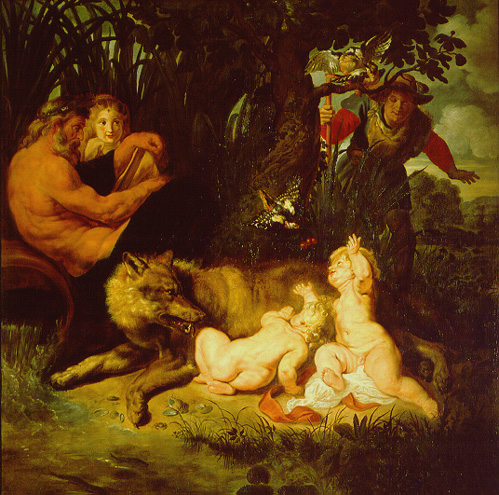
\includegraphics[scale=.3]{a20141211RaceandtheMythoftheOriginsofRome-img001.jpg} 
\end{wrapfigure}

The twins Romulus and Remus are abandoned to the waters and are saved from the waters. Here again is a symbolic theme recurring in many traditions: Moses is saved from the waters, the Indo-Aryan hero Karna is left in a basket in the river and is saved from the waters, and so on. But the symbol contained in the most ancient Aryan tradition is especially important, i.e., the Vedic tradition, in which ascetics are depicted as ``supreme natures who stand on the waters". Analogous explanations and, therefore, the hidden meaning of such a symbol, can be clarified as follows: the waters have traditionally always depicted the current of time, i.e., the basic element of mortal, unstable, contingent, passionate, fleeting life. The weak man is taken from the waters and carried from the waters. The seer or hero, the ascetic or the prophet is saved from the waters, or is capable of standing on the waters, or of not sinking in the waters. Hence, in the myth of the origins of Rome this symbol must again characterize the ``divine" element of the founders of Rome, their, so to speak, supernatural dignity.



\begin{quotex}
This is the second and concluding part of the essay by Julius Evola on the race and origins of Rome.

He points out the symbolism of fig tree, which was also the tree associated with the Buddha's awakening. The next symbol is the She-Wolf who suckles the twin babies. The wolf curiously has a dual symbolism: it can represent both the forces of light and the forces of darkness. This is often depicted as the battle between order, or Logos, with Chaos.

It is interesting to point out that the primal symbol of the wolf has been replaced in our time with the lap dog.

The spirit of Rome is exemplified by the manifestation ``of a principle of light and of order, of an ethic and a vision of life that is witness to the Aryan spirit". Here it is made clear that the Roman race is known through its spirit, not its genetics. So before constructing our Republic, it is necessary to describe that principle, ethic, and vision.

\end{quotex}
The twins find refuge near the fig tree [\emph{Ficus Ruminalis}] and are suckled by a She-wolf. The word Ruminal contains the idea of feeding: the quality of Ruminus, related to Jupiter, alluded to the quality of ``nourisher", of the ``god who gives nourishment" in the ancient Latin language. But this is the most elementary aspect of the symbol. In general, in the most ancient traditions of the Aryan races, the tree is the symbol of universal life, it is the tree of the world or the cosmic tree. If it is in form of a fig tree as it appears in the legend of Roman origins, precisely as a ``\emph{fico indico}" [Banyan tree] — the ashwattha tree — it is depicted as upside-down in the Indo-Aryan tradition to express that its roots are from above, in the ``heavens". The idea of a mystical food from the tree is a often recurring theme: the myth of Jason, Hercules, Odin, Gilgamesh, etc. Naturally, according to the races and their spirit, this then presents diverse variations. We know from the Hebraic myth that to pick and eat from the tree in order to make oneself like god is considered as the principle of guilt, abuse of power, and a curse. Things are conceived in a very different way in the myths of the Aryan races and even in the paleo-Chaldean myth of Gilgamesh. Also, in the legends of the Ghibelline Middle Ages, the heroic theme prevails and the tree often appears as that of the universal empire, reaching it in the symbolic lands of the mysterious Prester John means insuring the same dignity that the ancient Ario-Iranian rulers associated with the title of ``king of kings".

Returning to our main subject, in the myth of the twins at the origins of Rome, we therefore have the allusion to a supernatural food from the Tree — but also from the She-wolf. The symbol of the She-wolf, considered in its entirety and in all the stories that refer to it, has an ambiguous character. Lucian and Emperor Julian recall that, in the ancient world, on the basis of the phonetic resemblance between the two words, the idea of the wolf [\emph{lupo}] and of light [\emph{luce}] are often associated: \emph{lykos}, which in Greek means world, sound like \emph{lyke}, light. But there are also figurations of the wolf as a hellish animal, as a dark force. The Wolf thus appears to us in the double aspect, symbol of a ferocious and savage nature and also as the symbol of a luminous nature. This duality is verifiable, not only in Hellenic-Mediterranean prehistory, but also in the Celtic and Nordic. In fact, on the one hand in the Nordic-Celtic and Delphic cults the ``wolf" is connected to Apollo, i.e., to the Hyperborean, Nordic-Aryan god, simultaneously conceived as the solar god of the golden age and significantly associated by Virgil with Roman greatness. ``Sons of the wolf", on this basis, was a designation for warrior and heroic peoples of Nordic-Germanic origins, designations that persisted even to the epoch of the Goths and Nibelungs. Yet, on the other hand, in the Edda, the ``age of the Wolf" signifies a dark age, marking the epoch of the outbreak of savage and elementary forces, almost of the power of chaos, against the forces of the ``divine heroes", or Æsir.

Now we can certainly also relate this duality to the principle that, according to the legend of origins, ``fed" the two twins insofar as we see it reflected in their very nature, that is, in the antagonistic duality of Romulus and Remus, as related to us in the myth. As others already noticed, so also the theme of a single principle from which an antithesis is differentiated, whether depicted by the antagonism of two brothers of twins or, in general, of a couple, is found again in many traditions, and not rarely in respect to particularly significant moments for the origins of a given civilization, race, or religion. For example, we only recall that in the ancient Egyptian tradition Osiris and Set are two brothers of discord — sometimes conceived as twins—and one incarnates the luminous power of the sun, the other, a dark, ``infernal", principle, whose generation is called the ``sons of the impotent revolt". Does not something similar also show through perhaps in the Roman legend? Romulus is the one who marks the contour of the city as the meaning of a sacred rite and a principle of \emph{limit}—of order, of law—having received the right of putting his name to the city from the apparition of the solar number, of the \emph{twelve} vultures. Remus is instead the one who violates such a limit and is killed for this reason. One could say that the primordial force of Roman origins thus are differentiated and destroys the ``dark" powers that contained in themselves, affirms in its luminous aspect of order, Olympian domination, purified warrior force.

There have been attempts to see in the contrast between Romulus and Remus the reflection of the contrast between opposed Aryan racial forces, or of the Aryan type, and non-Aryan or pre-Aryan types. Research of this kind is without doubt interesting: problematic in its conclusions, if it intends to remain exclusively on the plane of material facts, or archeological and anthropological evidence. It has greater possibilities if it also penetrates the myth and legend in order to extract elements that integrate research in other domains. Naturally, in order to accomplish that, it also needs to resolve to outline general frameworks of various aspects of ancient Roman society, considering, for example, with various writers, somewhat probable that the social system of castes of ancient Rome had a racial substrate.

In this totality, it is interesting to examine the link between the two principles, whose symbolic figurations could well be Romulus and Remus, with the two hills Palatine and Aventine. The Palatine is, as we know, Romulus' hill and the Aventine is Remus'. Now, according to the ancient Italic tradition, on the Palatine, Hercules met the good king Evander (who significantly founded a temple of the goddess Victoria on the same Palatine hill) after having killed Cacus, son of the Pelasgian (pre-Aryan) god of the subterranean fire: and Hercules conquered and killed in Cacus' cave, \emph{located in the Aventine}, and erected an altar to the Olympic god, to whom he was allied according to the Hellenic myth. Researchers like Piganiol, are of the opinion that this duel between Hercules and Cacus — with the corresponding opposition of the Palatine and Aventine hills — could be a mythic transcription of the battle waged by peoples of opposing races.

The mythic legend of the origins of Rome is therefore saturated with deep meaning. The triumph of Romulus and the death of Remus is the key to the origin hidden in Romanity, and the first episode of a dramatic, outer and inner, spiritual, social and racial battle, in part known, in part still enclosed in symbols or in events not yet penetrated with respect to their most essential aspect, almost, we will say: with respect to the ``third dimension". Through this secular battle Rome rises gradually and asserts itself in the world as triumphal manifestations of a principle of light and of order, of an ethic and a vision of life that, in its original and uncorrupted forms, is witness to the Aryan spirit. And we know what it is, according to the most widespread tradition, the conclusion of the legend of origins: it is the apotheosis of Romulus, Romulus deified,

``he returned from the earth to heaven after his mortal part was destroyed by means of the dazzling fire."

So what has been treated is neither fantasy, nor poetry, nor rhetoric. Analogous explanations recur in the traditions of all peoples, according to a uniformity that should lead anyone to reflection. Also in regards to Romulus, the myth contains a faith and a spiritual certainty: it is the meaning of a reality that, freed from the person and symbol, was not once, but will always be, and will always be present, in its greatness beyond history, the race that knows how to recall the ``mystery".



\flrightit{Posted on 2014-12-08 by Aeneas }

\begin{center}* * *\end{center}

\begin{footnotesize}\begin{sffamily}



\texttt{Cologero on 2014-12-11 at 21:20 said: }

Tomberg quotes Hans Leisegang:

\begin{quotex}
Every myth expresses, in a form narrated for a particular case, an eternal idea which will be intuitively recognized by one who re-experiences the content of the myth. 

\end{quotex}
This is what Evola is getting at. So, of course, the myth ``contains" the eternal idea. Were it a simple reflection, then anyone could understand it. Rather, the idea is embedded, or hidden, in the myth, so it is discernible only to those who make the effort to re-experience it.


\hfill

\texttt{William Neville on 2014-12-13 at 01:51 said: }

Thank you for these translations, Cologero – this is valuable material.

It hadn't occurred to me before, but I wonder if Dante-specifically chose the She-Wolf as one of the beasts blocking the way out of the Dark Wood in the Divine Comedy as a reference to the She-Wolf in the story of Rome's founding. It would be interesting to meditate on and investigate.


\hfill


\hfill


\end{sffamily}\end{footnotesize}
